En el presente trabajo hemos explorado diferentes aristas relativas al problema de predicción planteado con el objetivo de responder nuestros interrogantes iniciales. 

% \begin{itemize}
%     \item El dataset de VarQ se concentra en variables de tipo estructural. ¿Podemos enriquecerlo con variables de otras dimensiones (físico-químicas, genómicas, filogenéticas)?
%     \item ¿Cómo afectan las distintas variables a nuestros modelos? ¿Cuáles son las más importantes?
%     \item ¿Cuáles son los mejores algoritmos de aprendizaje automático para resolver este tipo de problemas y cuáles son sus parámetros?
    
% \end{itemize}

La primer pregunta era acerca de la posibilidad de enriquecer el dataset con nuevas fuentes de datos. Esta pregunta fue respondida afirmativamente, dado que agregar nuevas dimensiones demostró ser efectivo en la mejora del modelo. 
En particular, el modelo que usó variables genómicas, arrojó un AUC de 0.85 (RF). El otro conjunto de variables analizado, las Físico-Químicas, también demostraron ser de utilidad, alcanzando un AUC de 0.72 (RF). El modelo Integral, que combinó ambos datasets, resultó ser superior a los anteriores. Luego sumar estas variables al dataset VarQ también mostró una mejora, pasando de un AUC de 0.74 a 0.88 (xgboost). Ver figuras \ref{fig:curvas_auc_humsavar} y \ref{fig:curvas_auc_varq}. [\todo{Faltan curvas de xgboost}]

Otra de las preguntas que nos hicimos al comienzo del trabajo, sobre la importancia de las variables, nos aportó información sobre como estas afectan al modelo, en el que detectamos en particular variables de conservación (phastCons y phyloP), la variación de la energía (del dataset varQ, obtenida vía PDB) y las matrices de sustitución o distancia (GRANTHAM, PAM250, BLOSUM, EX, JM y VB) como las más relevantes. Si bien el dataset VarQ ya poseía variables de conservación, estas pertenecen a familias de proteínas (Pfam).

Por último, pero no menos importante, este trabajo nos permitió comparar distintos métodos de aprendizaje automático, de los cuales obtuvimos los mejores resultados con métodos de ensamble, inicialmente con Random Forest y luego con el uso de xgboost para el modelo Integral. La descripción estadística del dataset nos permitió entender como el metodo tradicional para calcular importancia de variables en métodos de ensamble se ve afectado en variables altamente correlacionadas.  

\subsection{Trabajo Futuro}

Uno de los principales productos de este trabajo es la generación de un nuevo dataset que contiene numerosas variables estructurales y físico-químicos de la proteína, sumados a variables de tipo genómico. Este dataset también contiene variantes que están ligados a diferentes genes, que a su vez poseen cantidades distintas de SNPs potencialmente dañinos. Una de los trabajos que quedaron pendientes consisten en generar modelos individuales para cada gen, dado que puede existir un sesgo en nuestro modelo en caso de tener un número muy grande de SNPs de un gen determinado.

También creemos que los trabajos futuros que deriven de este deberían hacer énfasis en la generación de modelos que mejoren la selección de hiperparámetros (en particular sugerimos el uso de técnicas de optimización bayesiana), y un tratamiento de nulos en variables categóricas más avanzado en comparación al usado en este trabajo. 

\newpage

\begin{figure}[H]
\centering
\begin{subfigure}[b]{0.6\textwidth}
    \centering
    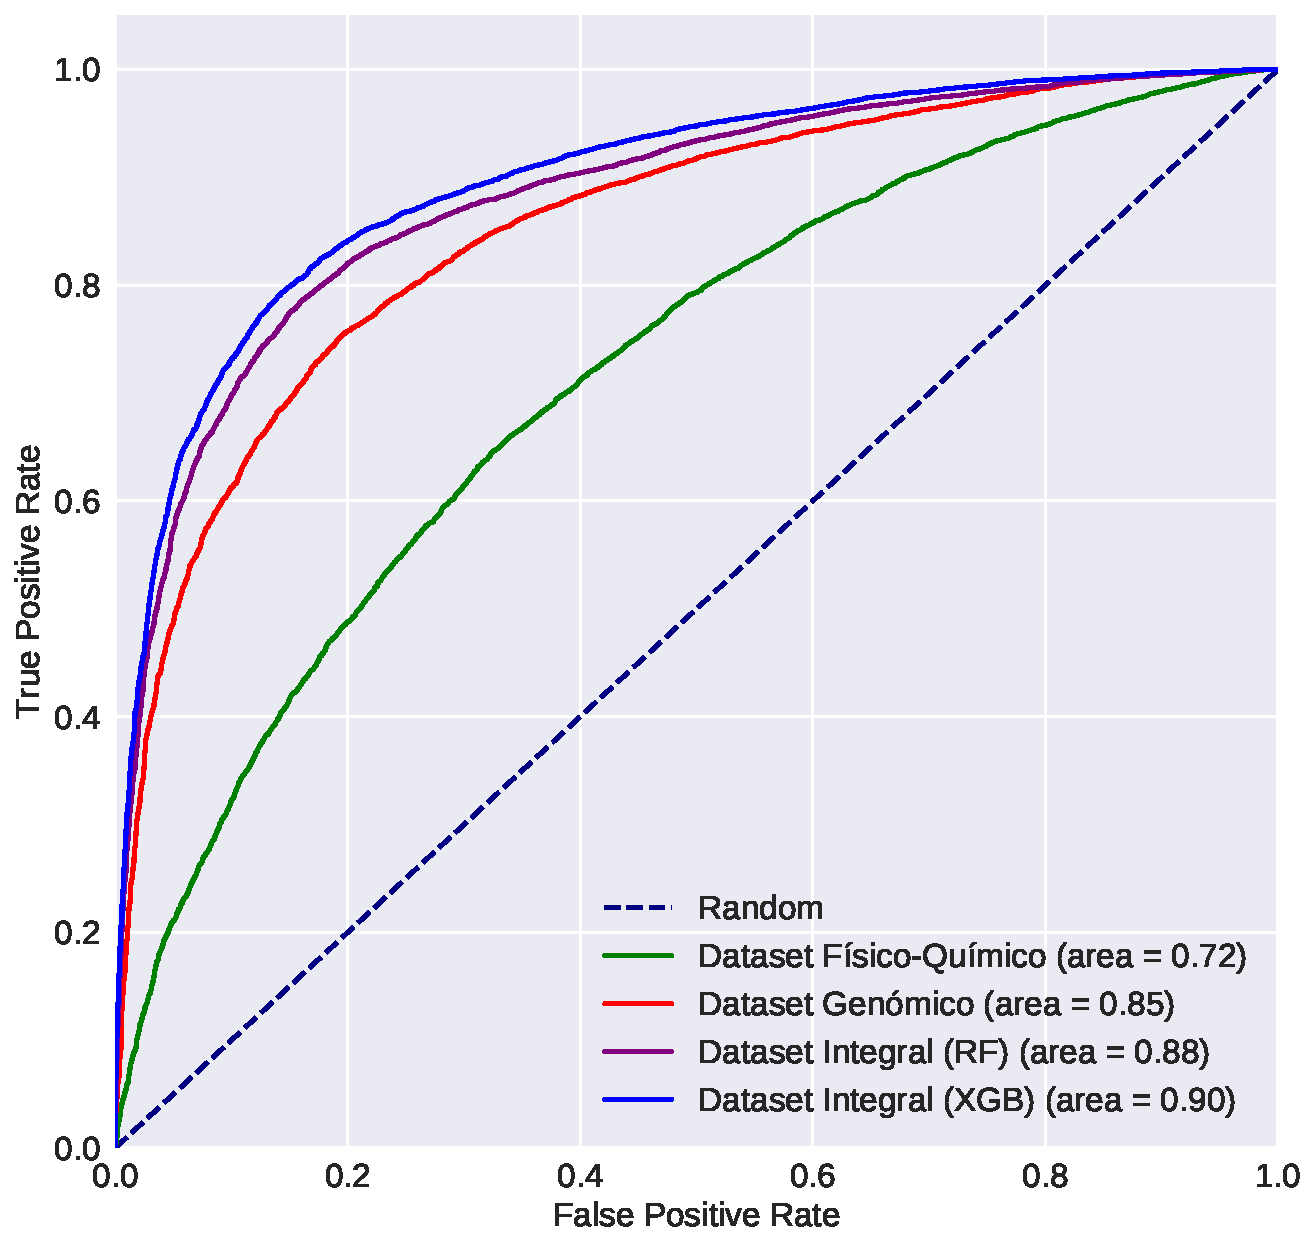
\includegraphics[width=\textwidth]{documents/latex/figures/4/curvas_auc_humsavar.pdf}
    \caption{Comparación de curvas ROC entre los datasets Físico-Químico, Genómico e Integral.}
    \label{fig:curvas_auc_humsavar}
\end{subfigure}

\hfill
\hfill

\begin{subfigure}[b]{0.6\textwidth}
    \centering
    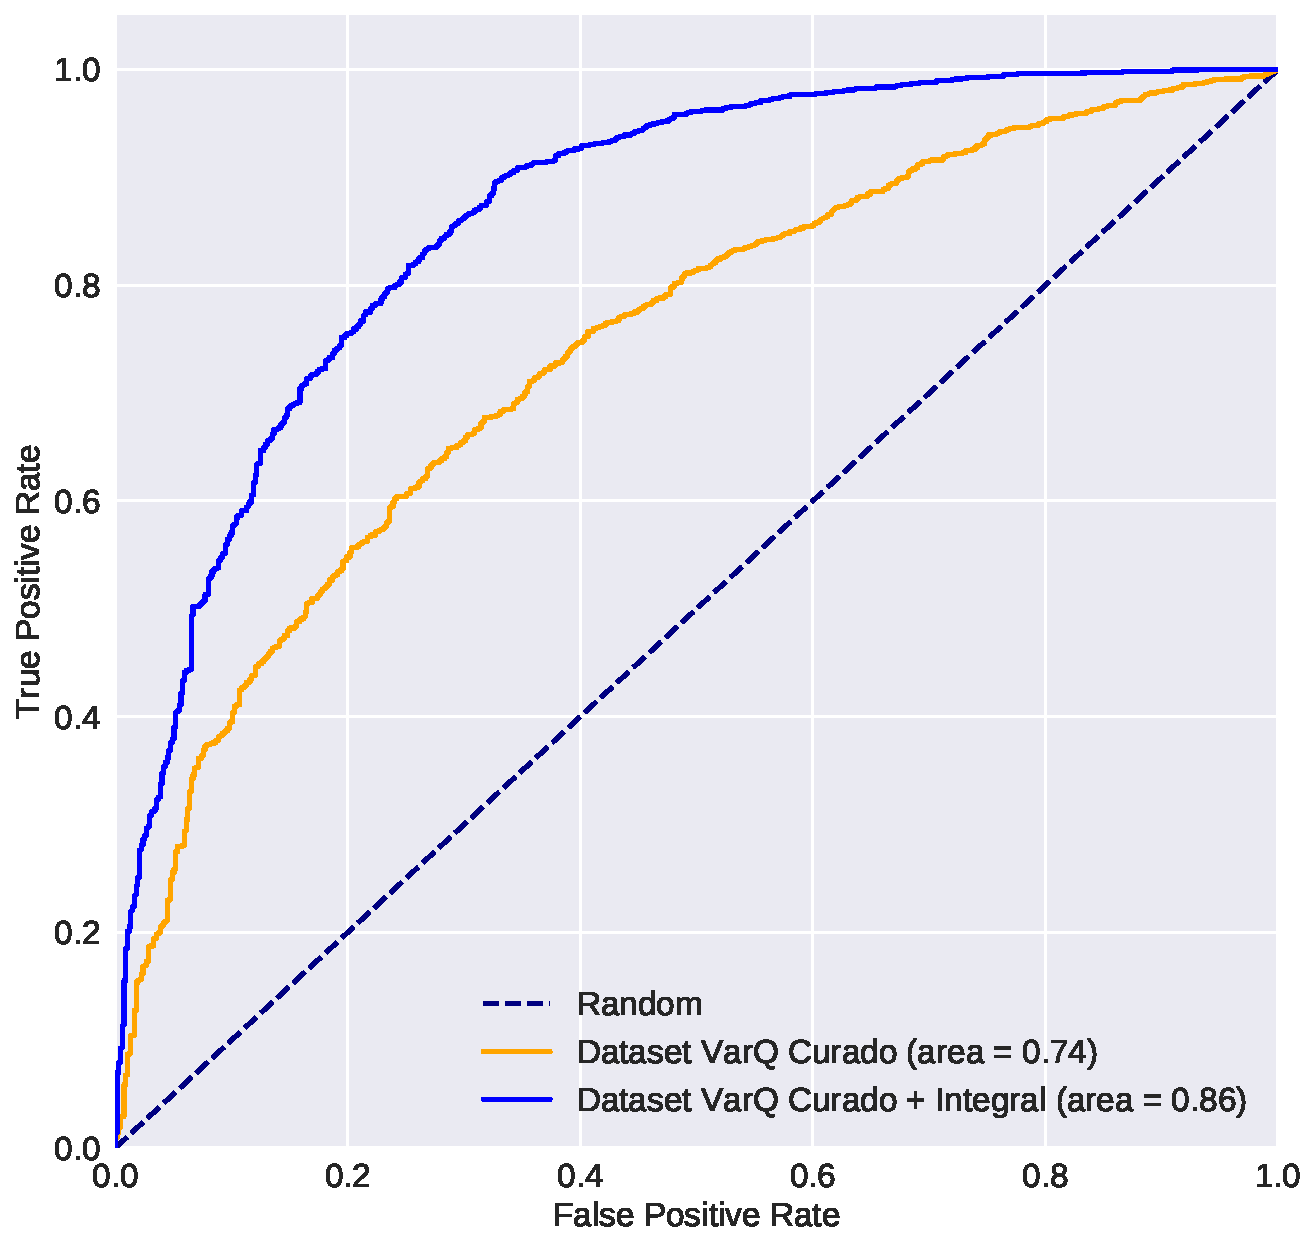
\includegraphics[width=\textwidth]{documents/latex/figures/4/curvas_auc_varq.pdf}
    \caption{Comparación de curvas ROC entre los datasets VarQ Curado y VarQ Curado + Integral.}
    \label{fig:curvas_auc_varq}
\end{subfigure}
\end{figure}


